\documentclass[9pt]{beamer}
\usetheme{Madrid}
\usepackage{mathtools}
\usepackage[T1]{fontenc}
\usepackage[english,french,spanish,italian]{babel}
\usepackage[useregional]{datetime2}
\usepackage{bm}
\usepackage{esvect}
\usepackage{amsmath}
\usepackage{physics}
\usepackage{empheq}
\usepackage[many]{tcolorbox}
\input{pool/NextDefs.tex}

%$\vv{\bm{L}}

\title{Krypton Calibration}
 
\subtitle{Run 6581}
 
\author{Krypton Calibration Group}
 
%\institute{Donostia International Physics Center (DIPC)} % (optional)
 
\date % (optional)
%{PHYSIS, SAN SEBASTIAN: 2-6 OCTOBER 2018}
 
%\logo{\includegraphics[height=0.5cm]{dipc.png}
%\includegraphics[height=0.5cm]{IB.png}}


\tcbset{highlight math style={enhanced,
  colframe=red!60!black,colback=yellow!50!white,arc=4pt,boxrule=1pt,
  }}

\newtcbox{\mybox}[1][]{nobeforeafter,math upper,tcbox raise base,
  enhanced,frame hidden,boxrule=0pt,interior style={top color=green!10!white,
  bottom color=green!10!white,middle color=green!50!yellow},
  fuzzy halo=1pt with green,drop large lifted shadow,#1}
  
%------------------------------------------------------------
%The next block of commands puts the table of contents at the 
%beginning of each section and highlights the current section:

%\AtBeginSection[]
%{
%  \begin{frame}
%    \frametitle{Table of Contents}
%    \tableofcontents[currentsection]
%  \end{frame}
%}
%------------------------------------------------------------

\begin{document}
\selectlanguage{english}
%The next statement creates the title page.
\frame{\titlepage}

%---------------------------------------------------------
%This block of code is for the table of contents after
%the title page

%\begin{frame}
%\frametitle{Table of Contents}
%\tableofcontents
%\end{frame}

%---------------------------------------------------------


%\section{Run 6581}

%---------------------------------------------------------

\begin{frame}
\frametitle{Conditions and data}

\begin{table}[h!]
\caption{Conditions and data for run 6581}
\begin{center}
\begin{tabular}{|c|c|}
\hline
Conditions & Data \\
\hline
run number & 6581 \\
file range & (0,6680) \\
date & December 30th \\
lab temperature: & 20 $\deg$ \\
Total number of S2s  &  2328327 \\
Total number of events & 2015406 \\
\hline
\end{tabular}
\end{center}
\label{r6581.data}
\end{table}%
\end{frame}

\begin{frame}
\begin{figure}
  \begin{center}
      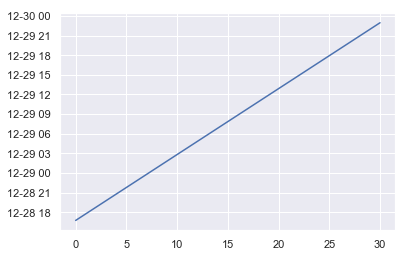
\includegraphics[width=0.45\textwidth]{img/r6581/runTime.png}
      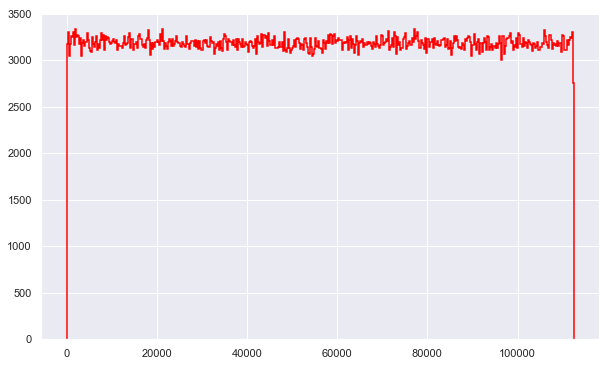
\includegraphics[width=0.45\textwidth]{img/r6581/runEvt.png}
    \caption{Run data.}
  \end{center}
\end{figure}
\end{frame}

\begin{frame}
\frametitle{S1 \& S2}

\begin{table}[h!]
\caption{S1 \& S2 for run 6581}
\begin{center}
\begin{tabular}{|c|c|}
\hline
Conditions & Data \\
\hline
fraction of S1s & 0.79 \\
fraction of S2s (1 S1) & 0.97 \\
fraction 1 S2 \& 1 S1 & 0.77 \\
\hline
\end{tabular}
\end{center}
\label{r6581.data}
\end{table}%

\begin{table}[h!]
\caption{S1 \& S2 selection for run 6581}
\begin{center}
\begin{tabular}{|c|c|}
\hline
Variables & Data \\
\hline
$s_1$~energy & \SIrange{3}{25}{pes} \\
$s_2$~energy (PMTs) & \SIrange{3000}{14000}{pes}\\
$s_2$~charge (SiPMs) & \SIrange{300}{800}{pes}\\
$s_2$~width & \SIrange{5}{15}{\micro\second}\\
$n_{sipm}$~min & 15\\
\hline
\end{tabular}
\end{center}
\label{r6581.sel}
\end{table}%
\end{frame}


\begin{frame}
\begin{figure}
  \begin{center}
      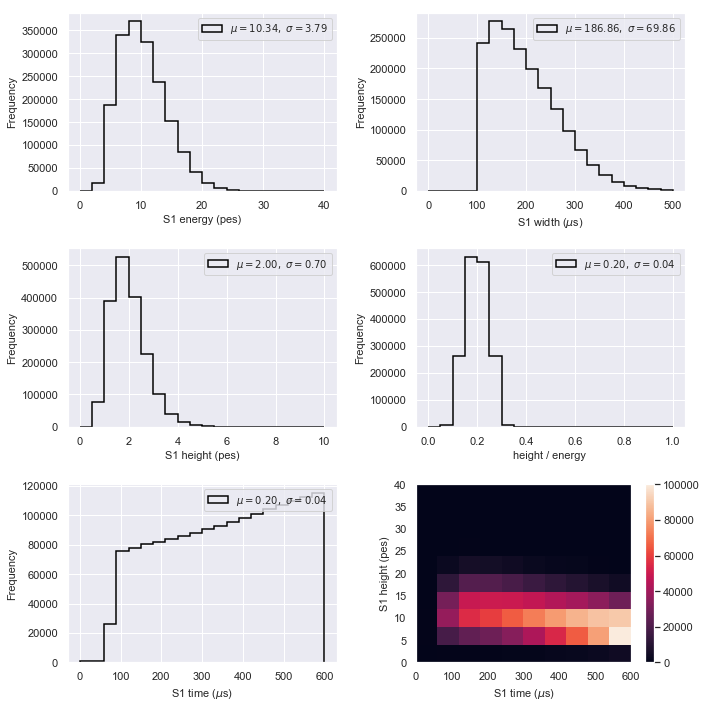
\includegraphics[width=0.6\textwidth]{img/r6581/s1.png}
    \caption{S1 distributions.}
  \end{center}
\end{figure}
\end{frame}

\begin{frame}
\begin{figure}
  \begin{center}
      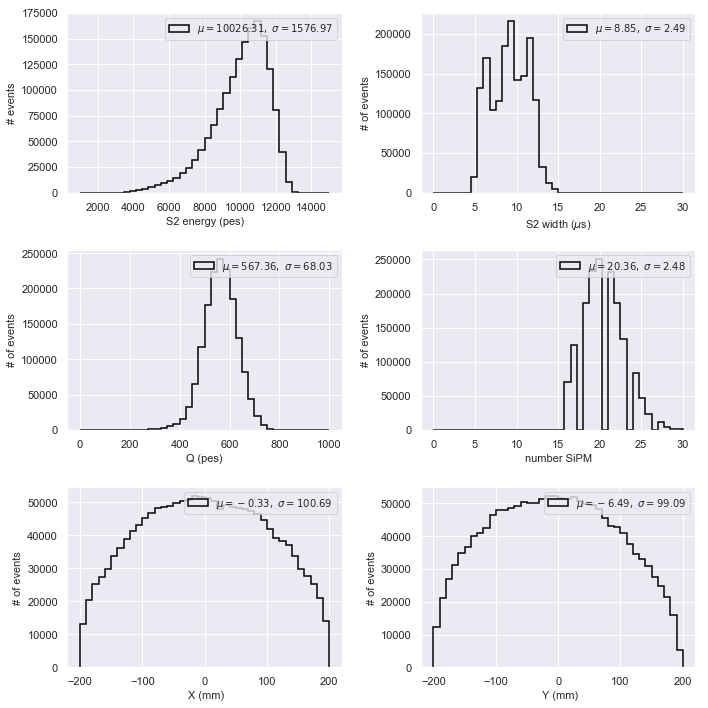
\includegraphics[width=0.6\textwidth]{img/r6581/s2.png}
    \caption{S2 distributions.}
  \end{center}
\end{figure}
\end{frame}

\begin{frame}
\frametitle{Control distributions}
\begin{figure}
  \begin{center}
      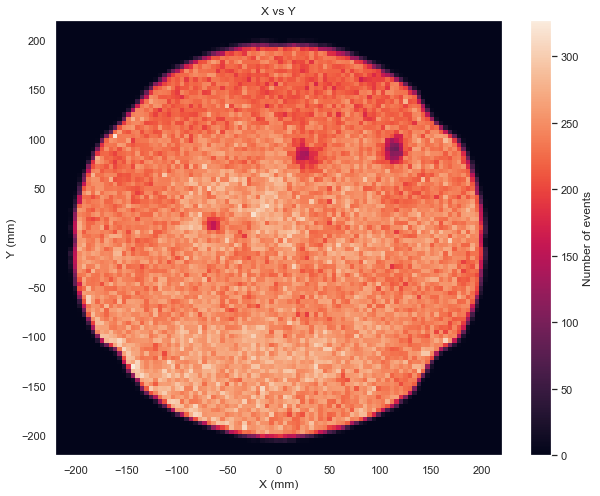
\includegraphics[width=0.6\textwidth]{img/r6581/xy.png}
    \caption{XY distribution.}
  \end{center}
\end{figure}
\end{frame}

\begin{frame}
\begin{figure}
  \begin{center}
      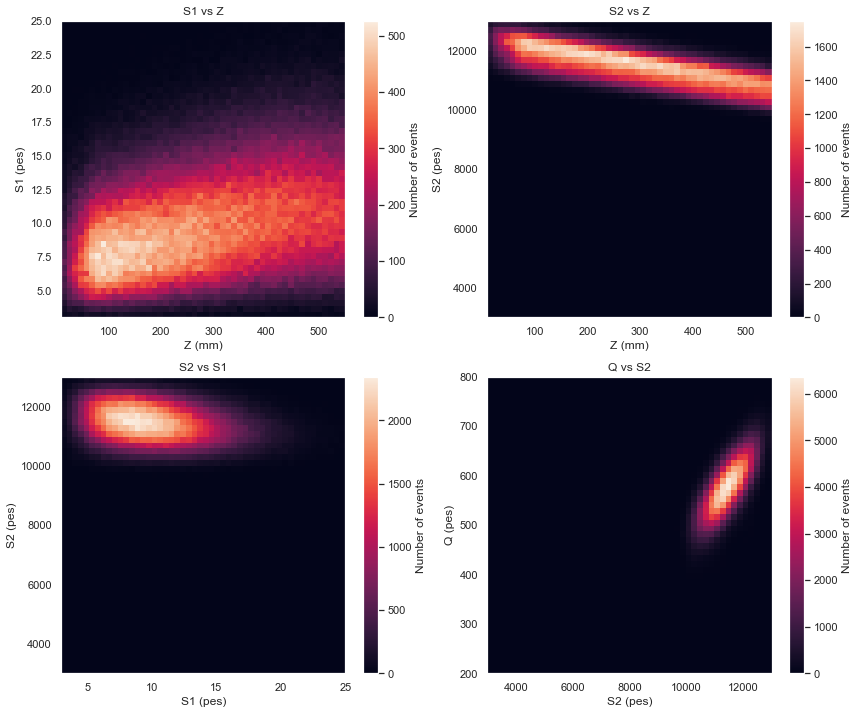
\includegraphics[width=0.7\textwidth]{img/r6581/s1s2q.png}
    \caption{S1, S2 \& Q distributions.}
  \end{center}
\end{figure}
\end{frame}

\begin{frame}
\frametitle{Lifetime distributions}
\begin{figure}
  \begin{center}
      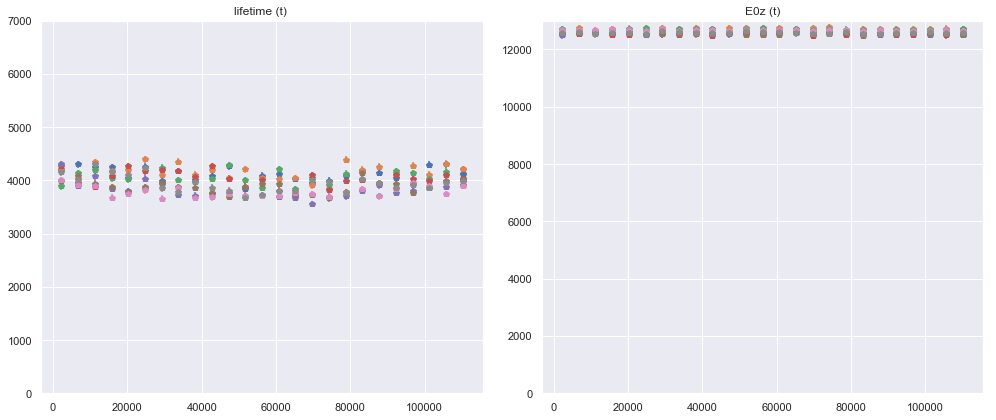
\includegraphics[width=0.4\textwidth]{img/r6581/R_phi_lt1.png}
      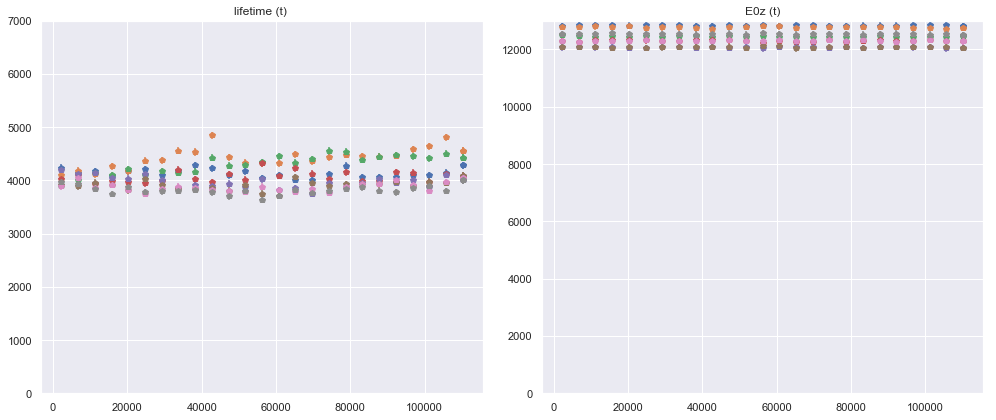
\includegraphics[width=0.4\textwidth]{img/r6581/R_phi_lt2.png} \\
      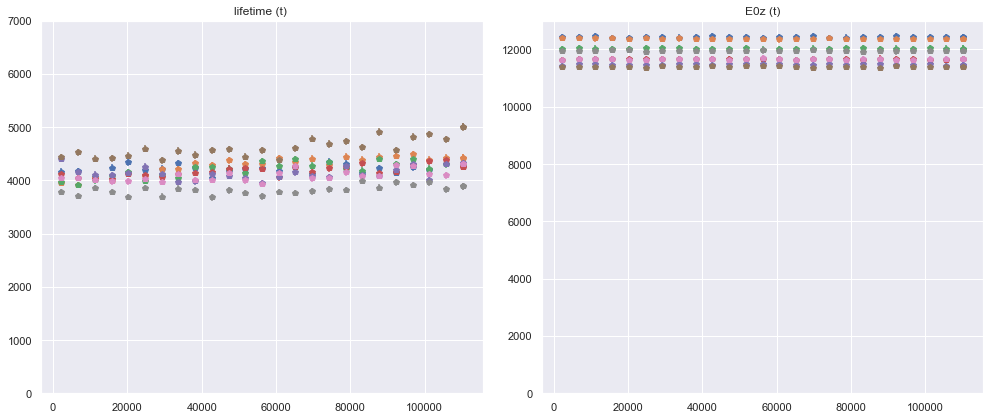
\includegraphics[width=0.4\textwidth]{img/r6581/R_phi_lt3.png}
      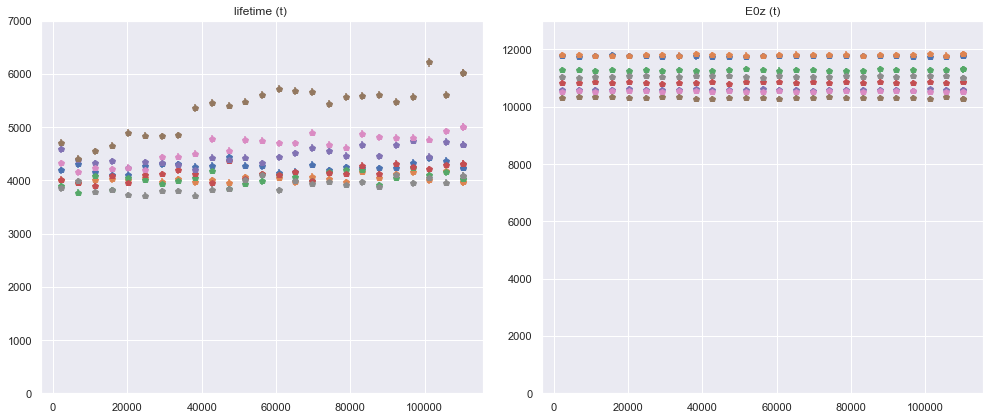
\includegraphics[width=0.4\textwidth]{img/r6581/R_phi_lt4.png}\\
      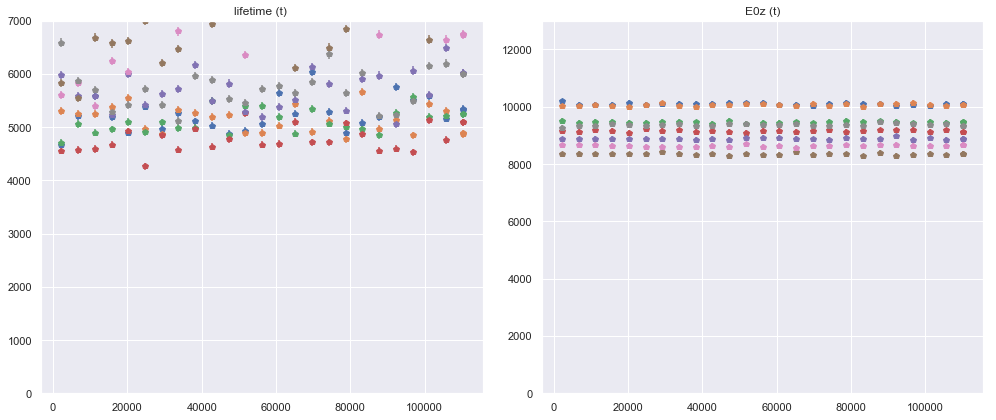
\includegraphics[width=0.4\textwidth]{img/r6581/R_phi_lt5.png}
    \caption{Distributions of lifetime and $E_0$~for 5 radial sectors (40, 80, 120, 160, 200).}
  \end{center}
\end{figure}
\end{frame}

\begin{frame}
\frametitle{Lifetime maps}
\begin{figure}
  \begin{center}
      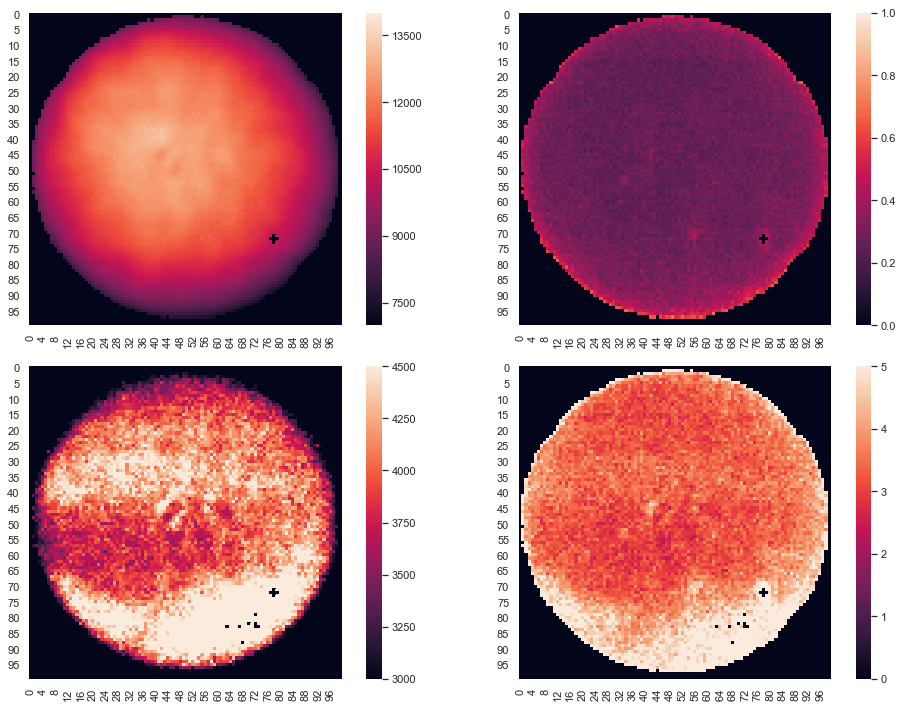
\includegraphics[width=0.7\textwidth]{img/r6581/maps.png}
    \caption{Lifetime and geometrical map.}
  \end{center}
\end{figure}
\end{frame}

\begin{frame}
\frametitle{Lifetime maps}
\begin{figure}
  \begin{center}
      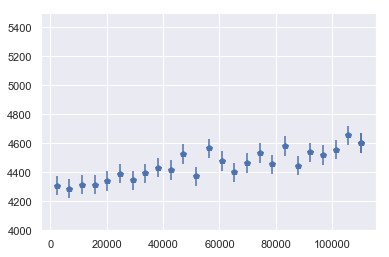
\includegraphics[width=0.7\textwidth]{img/r6581/AverageLT.png}
    \caption{Average lifetime.}
  \end{center}
\end{figure}
\end{frame}

\begin{frame}
\frametitle{Lifetime and geometry correction}
\begin{figure}
  \begin{center}
      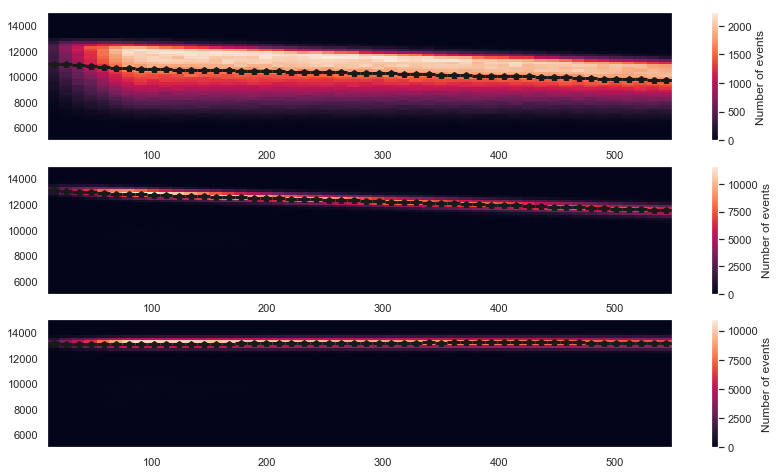
\includegraphics[width=0.7\textwidth]{img/r6581/CorrectionLT.png}
    \caption{Lifetime and geometry correction.}
  \end{center}
\end{figure}
\end{frame}

\begin{frame}
\frametitle{R Profile showing R dropout}
\begin{figure}
  \begin{center}
      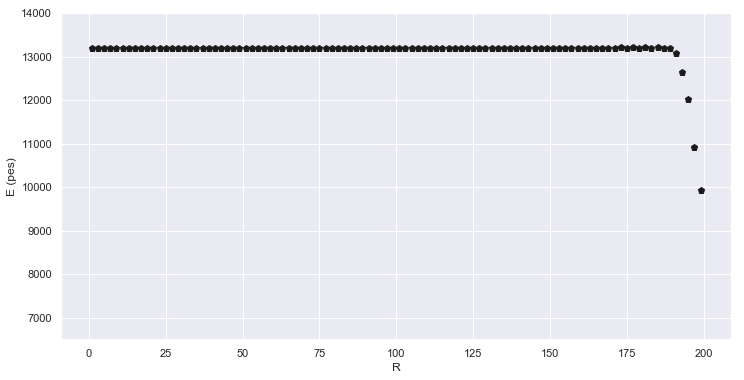
\includegraphics[width=0.7\textwidth]{img/r6581/RProfile.png}
    \caption{R profile shows that fiducial volume must be $R < 180$mm.}
  \end{center}
\end{figure}
\end{frame}


\begin{frame}
\frametitle{Profiles after $R < 180$mm}
\begin{figure}
  \begin{center}
      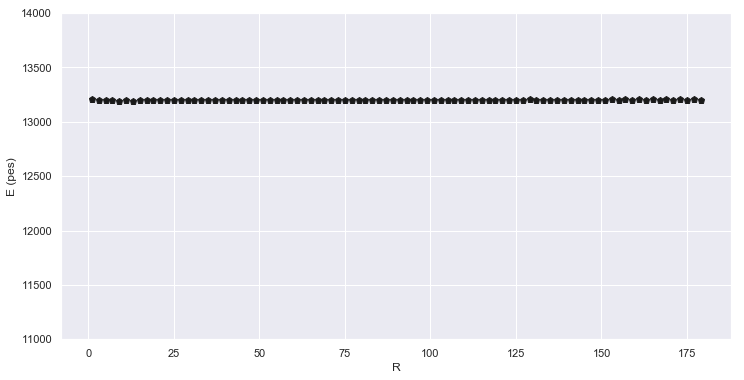
\includegraphics[width=0.4\textwidth]{img/r6581/RProfileC.png}
      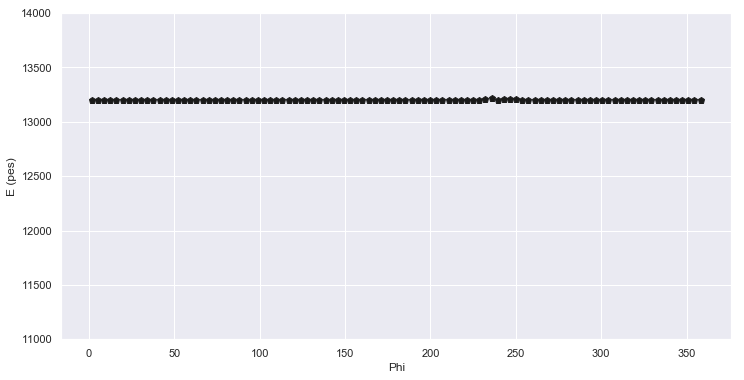
\includegraphics[width=0.4\textwidth]{img/r6581/PhiProfile.png} \\
      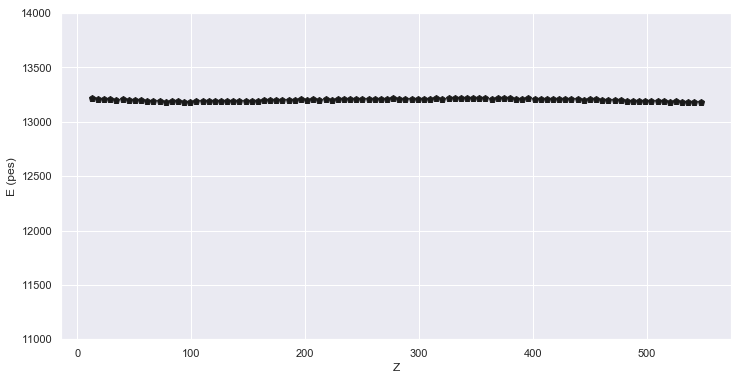
\includegraphics[width=0.4\textwidth]{img/r6581/ZProfile.png}
      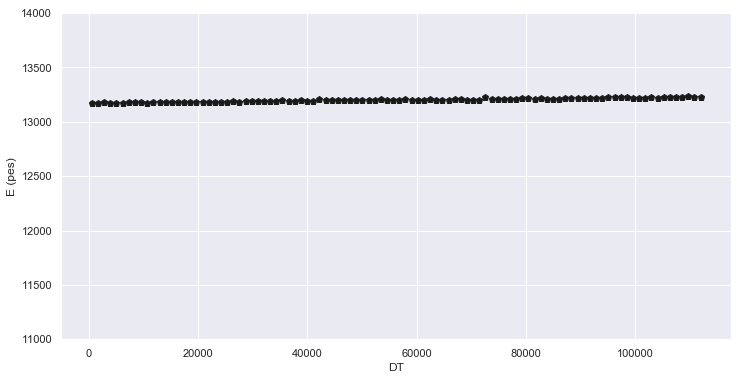
\includegraphics[width=0.4\textwidth]{img/r6581/TProfile.png}
    \caption{Profiles showing correction is robust.}
  \end{center}
\end{figure}
\end{frame}

\begin{frame}
\frametitle{Resolution fits as a function of R and Z}
\begin{figure}
  \begin{center}
      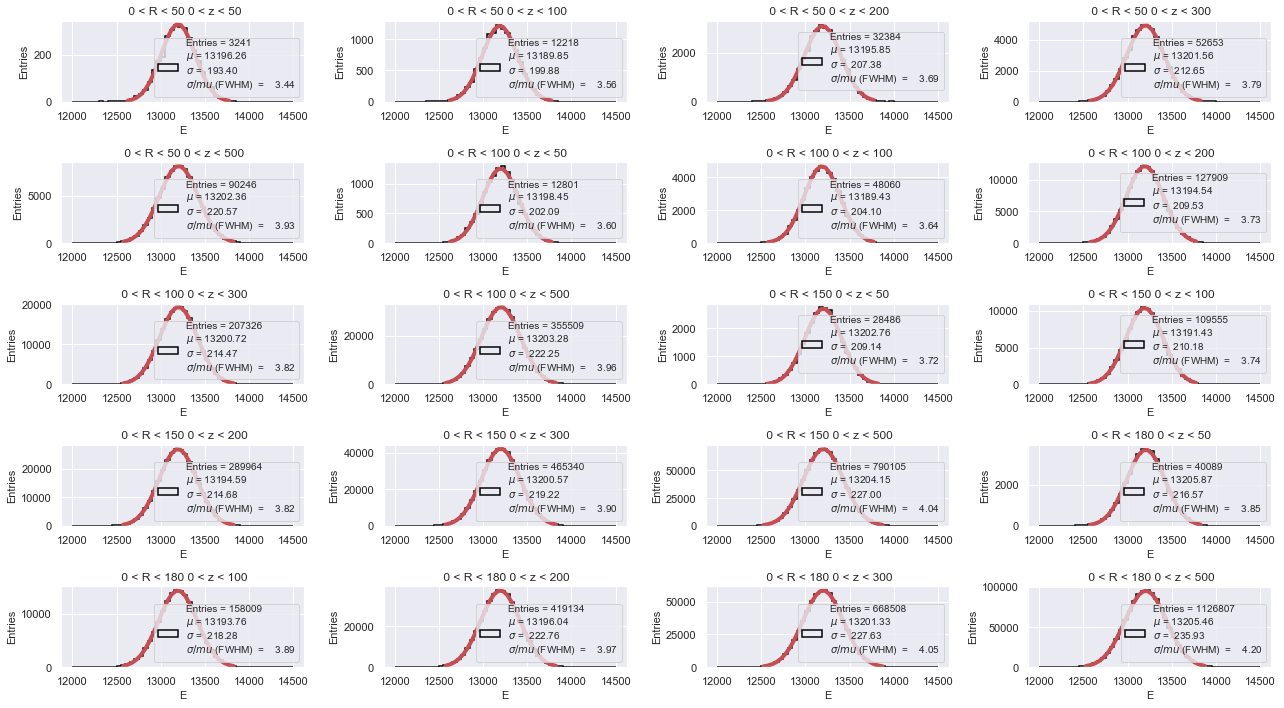
\includegraphics[width=0.8\textwidth]{img/r6581/ResoFit.png}
    \caption{Resolution fits.}
  \end{center}
\end{figure}
\end{frame}

\begin{frame}
\frametitle{Resolution as a function of R and Z}
\begin{figure}
  \begin{center}
      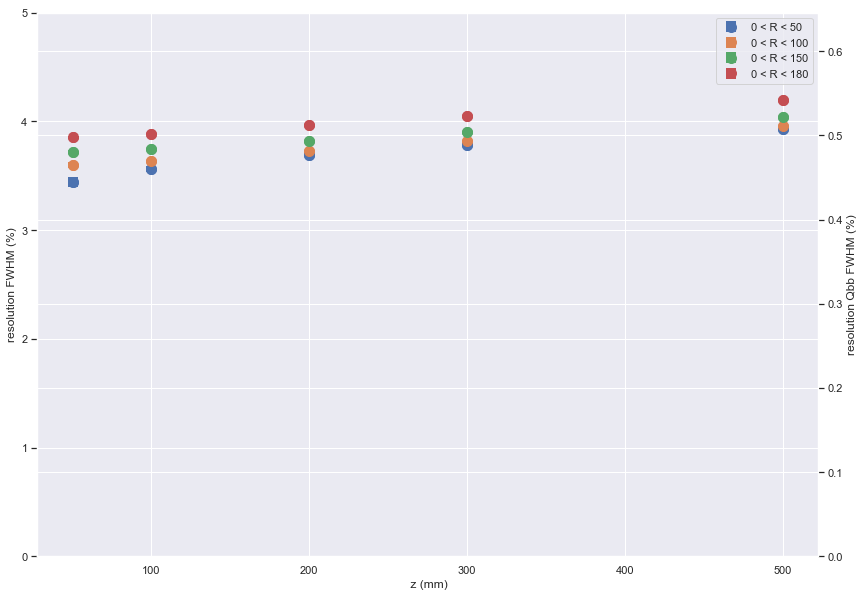
\includegraphics[width=0.8\textwidth]{img/r6581/ResoVsZR.png}
    \caption{Resolution fits.}
  \end{center}
\end{figure}
\end{frame}






%\section{Run 6582}
%\input{slides/run6582.tex}



\end{document}